\documentclass[titlepage,12pt]{article}

\usepackage[utf8]{inputenc}
\usepackage[brazil]{babel}
\usepackage[T1]{fontenc}
\usepackage{url}
\usepackage{verbatim}
\usepackage{xspace}
\usepackage{graphicx}

\begin{comment}
Responsibility in the project:
(in portuguese)

- Liderança técnica do projeto.
- Desenvolvimento das partes mais críticas do projeto relacionadas ao design do
  linguagem de programação.
- Orientação de alunos de graduação e mestrado.

Responsibility in the project:
(in english)

- Technical leadership.
- Development of the most critical parts of the project related to the design
  of the programming language.
- Supervising students.

\end{comment}

\newcommand{\CEU}{\textsc{C\'{e}u}\xspace}

\title{ Uma Plataforma Flexível, Barata e de Baixo Consumo Energético para a
        Internet das Coisas }

\author{PROPONENTE:                                     \\
Francisco Figueiredo Goytacaz Sant'Anna                 \\
francisco@ime.uerj.br                                   \\
\\\\
INSTITUIÇÃO DE EXECUÇÃO:                                \\
Universidade Estadual do Rio de Janeiro (UERJ)          \\
\\\\
Chamada Universal MCTIC/CNPq 2018 
}

\begin{document} 

\maketitle

%\begin{abstract} \end{abstract}

%%%%%%%%%%%%%%%%%%%%%%%%%%%%%%%%%%%%%%%%%%%%%%%%%%%%%%%%%%%%%%%%%%%%%%%%%%%%%%%
% a) Identificação do projeto, incluindo título, palavras-chave e resumo;
%%%%%%%%%%%%%%%%%%%%%%%%%%%%%%%%%%%%%%%%%%%%%%%%%%%%%%%%%%%%%%%%%%%%%%%%%%%%%%%

\section{Identificação do Projeto}

\subsection{Título}

Uma Plataforma Flexível, Barata e de Baixo Consumo Energético para a Internet
das Coisas

%A Low-Power, Flexible, and Cheap Platform for the Internet of Things

\subsection{Palavras-Chave}

internet das coisas, eficiência energética, linguagem de programação síncrona

%iot, arduino, low power, synchronous language

\subsection{Resumo}

De acordo com a Agência Internacional de Energia (AIE)~\cite{iea.data}, o
número de dispositivos conectados em rede deve atingir 50 bilhões até 2020 com
a expansão da Internet das Coisas (IoT).
A maior parte do consumo de energia nesses dispositivos será em
\emph{modo de espera} (aka \emph{standby mode}), quando eles não estão
transmitindo ou processando dados ativamente.
Atualmente, o modo de espera é responsável por 10 a 15\% do consumo
residencial.
Também estima-se que as emissões globais de $CO_2$ relacionadas ao modo de
espera seja equivalente às emissões de 1 milhão de carros.

Os efeitos do consumo de energia sobre o meio ambiente, aliados ao grande
crescimento da IoT no curto prazo, tornou o modo de espera para dispositivos
conectados um dos seis pilares do \emph{Plano de Ação para Eficiência
Energética do G20}%
\footnote{G20's Energy Efficiency Action Plan: \url{https://www.iea-4e.org/projects/g20}}.
No entanto, o uso efetivo do modo de espera requer grandes esforços de hardware
e software para detectar períodos de inatividade nos dispositivos, identificar
periféricos que devem (ainda) permanecer ligados, e aplicar os modos de energia
mais econômicos sempre que possível.

Este projeto tem como principal objetivo desenvolver uma plataforma de hardware
e software de baixo consumo de energia para pesquisa e educação em Internet das
Coisas.

No que diz respeito ao software, iremos adotar a linguagem de programação
reativa \CEU~\cite{ceu.sensys13}, a qual estamos desenvolvendo durante os
últimos 8 anos, e que tem como alvo sistemas embarcados e a IoT.
%
\CEU é baseada no modelo de concorrência síncrono, no qual todas as reações ao
mundo externo são computadas em tempo finito, garantindo que as aplicações
sempre cheguem a um estado ocioso suscetível ao modo de espera.
%
A linguagem já possui suporte recente ao gerenciamento automático de energia.
Em testes preliminares, alcançamos economias entre 20 e 90\% para aplicações
escritas puramente em \CEU.

No que diz respeito ao hardware, iremos adotar microcontroladores e
transceptores de rádio de baixo consumo de energia.
Além disso, buscamos como requisitos extras o baixo custo e flexibilidade da
plataforma para maior adequação ao contexto de pesquisa e educação.
%
As soluções completas de hardware para IoT atuais são pouco flexíveis, pois
tipicamente possuem componentes SMD já soldados às placas.
Em particular, os módulos de rádio são pré-determinados, criando uma barreira
para a experimentação.
Mesmo havendo soluções abertas, o método de montagem industrial tipicamente
adotado não é adequado para pesquisa e educação.
%
A nossa proposta visa projetar uma solução flexível e de baixo custo baseada em
microcontroladores e módulos ``de prateleira'' do mercado brasileiro.

%%%%%%%%%%%%%%%%%%%%%%%%%%%%%%%%%%%%%%%%%%%%%%%%%%%%%%%%%%%%%%%%%%%%%%%%%%%%%%%
% b) Dados do proponente e equipe;
% d) Instituição(ões) participante(s);
%%%%%%%%%%%%%%%%%%%%%%%%%%%%%%%%%%%%%%%%%%%%%%%%%%%%%%%%%%%%%%%%%%%%%%%%%%%%%%%

\section{Equipe e Instituições}

\begin{itemize}
    \item Francisco Figueiredo Goytacaz Sant'Anna
    \begin{itemize}
        \item \textbf{Função:} \\
              Pesquisador Proponente e Coordenador
        \item \textbf{E-mail:} \\
              \url{francisco@ime.uerj.br}
        \item \textbf{Lattes:} \\
              \url{http://lattes.cnpq.br/0077491494754494}
        \item \textbf{Instituição:}                                     \\
              Departamento de Informática e Ciências da Computação      \\
              Programa de Pós-Graduação em Engenharia Eletrônica (PEL)  \\
              Universidade Estadual do Rio de Janeiro (UERJ)
    \end{itemize}

    \item Alexandre Sztajnberg
    \begin{itemize}
        \item \textbf{Função:} \\
              Pesquisador Colaborador
        \item \textbf{E-mail:} \\
              \url{alexszt@ime.uerj.br}
        \item \textbf{Lattes:} \\
              \url{http://lattes.cnpq.br/0403732822984772}
        \item \textbf{Instituição:}                                     \\
              Departamento de Informática e Ciências da Computação      \\
              Programa de Pós-Graduação em Engenharia Eletrônica (PEL)  \\
              Universidade Estadual do Rio de Janeiro (UERJ)
    \end{itemize}
\end{itemize}

%%%%%%%%%%%%%%%%%%%%%%%%%%%%%%%%%%%%%%%%%%%%%%%%%%%%%%%%%%%%%%%%%%%%%%%%%%%%%%%
% c) Área(s) do conhecimento predominante(s);
%%%%%%%%%%%%%%%%%%%%%%%%%%%%%%%%%%%%%%%%%%%%%%%%%%%%%%%%%%%%%%%%%%%%%%%%%%%%%%%

\section{Áreas de Conhecimento}

\begin{itemize}
\item Área predominante:
    \begin{itemize}
    \item Ciência da Computação --- Sistemas de Computação     
    \end{itemize}
\item Áreas relacionadas:
    \begin{itemize}
    %\item Engenharia de Telecomunicações --- Sistemas de Telecomunicações
    \item Ciência da Computação --- Linguagens de Programação
    \item Outra --- Microeletrônica --- Projeto
    \end{itemize}
\end{itemize}

%%%%%%%%%%%%%%%%%%%%%%%%%%%%%%%%%%%%%%%%%%%%%%%%%%%%%%%%%%%%%%%%%%%%%%%%%%%%%%%
% e) Objetivos geral e específicos;
%%%%%%%%%%%%%%%%%%%%%%%%%%%%%%%%%%%%%%%%%%%%%%%%%%%%%%%%%%%%%%%%%%%%%%%%%%%%%%%

\section{ Objetivos }

\subsection{ Objetivos Gerais }

Criar uma plataforma de hardware e software para pesquisa e educação em
Internet das Coisas que seja flexível, barata e de baixo consumo energético.

\subsection{ Objetivos Específicos }

A plataforma deve alcançar os seguintes objetivos:

\begin{description}
%
\item[Baixo Consumo Energético:]
  O hardware deve possuir modos de economia de energia para todos os seus
  componentes, sejam eles o microcontrolador, sensores ou módulos de rádio.
  O software será baseado em uma linguagem de programação ciente de energia.
  A linguagem deve ser capaz de detectar quando os componentes estão ociosos
  para colocá-los em modo de espera automaticamente, sem a intervenção do
  programador.
%
\item[Flexível:]
  O hardware deve prever conexões para uma variedade de sensores e
  transceptores de rádio frequência.
  Em particular, os módulos de rádio mais populares devem ser todos acopláveis
  externamente ao hardware.
  O software deve ser modular, de maneira que somente os drivers dos
  dispositivos de interesse sejam compilados junto com as aplicações.
%
\item[Barata:]
  O hardware deve usar microcontroladores e módulos ``de prateleira'' comuns no
  mercado para compras em pequenas quantidades e a custo baixo.
  O plataforma de software deve ser \emph{open source}.
%
\end{description}

Como principais desafios, o hardware deve possuir mecanismos flexíveis que
permitam desabilitar periféricos via software e, principalmente, o software
deve oferecer mecanismos automáticos para colocar o hardware em modo de espera,
sem esforços extras por parte do programador.

\begin{comment}

To create a hardware and software platform for research and education in IoT
that is flexible, cheap, and low power.

The platform should achieve the following objectives:

- Low power consumption:

The hardware should provide low-power mode for all of its components, such as
the microcontroller, sensors, and radio modules.
The software will be based on an energy-aware programming language.
The language should be able to detect when the components are idle in order to
put them in standby mode automatically, without intervention from the
programmer.

- Flexible:

The hardware should provide connections for a variety of sensors and radio
transceivers.
In particular, the most popular radio modules should all be attachable
externally the hardware.
The software should be modular in such a way that only the drivers from
peripherals in use are compiled with the applications.

- Cheap:

The hardware should use off-the-shelf microcontrollers and modules that are
typical in the market to buy in small quantities and at low cost.
The software platform should be open source.

As the main challenges, the hardware should provide flexible mechanisms to
allow disabling peripherals via software, and the software should provide
automatic mechanisms to put the hardware in standby without programmer
intervention.

\end{comment}

\begin{comment}
O enfoque principal se dá no baixo consumo de energia, mas a flexibilidade e
baixo custo são fundamentais para promover uma maior adoção da plataforma,
principalmente no contexto de pesquisa em IoT.
\end{comment}

%%%%%%%%%%%%%%%%%%%%%%%%%%%%%%%%%%%%%%%%%%%%%%%%%%%%%%%%%%%%%%%%%%%%%%%%%%%%%%%
% f) Metodologia proposta;
%%%%%%%%%%%%%%%%%%%%%%%%%%%%%%%%%%%%%%%%%%%%%%%%%%%%%%%%%%%%%%%%%%%%%%%%%%%%%%%

\section{Metodologia}

O projeto possui duas linhas concomitantes de pesquisa---em \emph{software} e
em \emph{hardware}---que se complementam para oferecer uma plataforma completa,
mas que também são suficientemente independentes para serem desenvolvidas o
máximo em separado.

\subsection{Software}
\label{sec.metodologia.software}

Grande parte da pesquisa em software está fundamentada em trabalhos anteriores
nossos com a linguagem \CEU~\cite{ceu.sensys13,ceu.tecs17,ceu.lctes18}.
A linguagem já possui uma implementação estável e foi adotada com sucesso nas
áreas de redes de sensores sem fio~\cite{ceu.sensys13,ceu.terra},
jogos~\cite{ceu.mod15} e multimídia~\cite{ceumedia.webmedia16}.

Mais recentemente, investigamos como prover tratamento de interrupções e
gerenciamento automático do modo de espera diretamente em \CEU, já obtendo
resultados preliminares com baixo consumo de energia~\cite{ceu.lctes18.short}.
%
No entanto, a plataforma de software proposta neste projeto requer uma pesquisa
mais extensa, que ainda deve abranger os seguintes temas:
%
\begin{enumerate}
\item Avaliação qualitativa da usabilidade de \CEU.
\item Avaliação quantitativa do uso de recursos de \CEU, tais como memória,
      desempenho e, principalmente, consumo de energia.
\item Desenvolvimento de aplicações representativas de IoT que usem comunicação
      por rádio extensivamente.
\item Cobertura de drivers para periféricos e módulos de rádio diversos.
\end{enumerate}

O coordenador do projeto ficará responsável pelas partes mais críticas da
pesquisa, tais como o funcionamento da linguagem e dos drivers para os
periféricos mais essenciais (item 4).

Uma aluna de mestrado está trabalhando em um ambiente de programação
educacional para IoT que tem como alvo alunos no início da graduação em Ciência
da Computação.
Nossa hipótese é que o vocabulário especializado de \CEU para lidar com o mundo
externo (e.g., eventos e concorrência) irá permitir que os alunos desenvolvam
projetos de IoT simples mas completos.
Essa frente de pesquisa será importante para a avaliação de usabilidade da
linguagem (item 1).

O desenvolvimento de aplicações IoT completas (item 3) é fundamental para
validar o projeto como um todo.
A Internet oferece diversas aplicações de IoT abertas e disponíveis que poderão
servir como base para as avaliações qualitativas e quantitativas (itens 2 e 3).
Alunos de iniciação científica e projeto final poderão trabalhar em projetos
diferentes que servirão para essas avaliações de \CEU.

\subsection{Hardware}

A nossa proposta visa projetar uma solução de hardware flexível e de baixo
custo baseada em microcontroladores e módulos ``de prateleira'' no mercado
brasileiro com os seguintes requisitos:
%
\begin{enumerate}
\item O microcontrolador deve possuir baixo consumo de energia e oferecer
      modos de espera programáveis.
\item Os módulos de rádio mais populares devem ser acopláveis externamente ao
      hardware para experimentação de diversas propriedades de RF, tais como
      técnica de modulação, alcance, velocidade, interoperabilidade, etc.
\item O hardware deve possuir mecanismos que permitam desabilitar sensores e
      periféricos via software para maximizar a economia de energia.
\end{enumerate}

\begin{figure}
\begin{minipage}{0.50\textwidth}
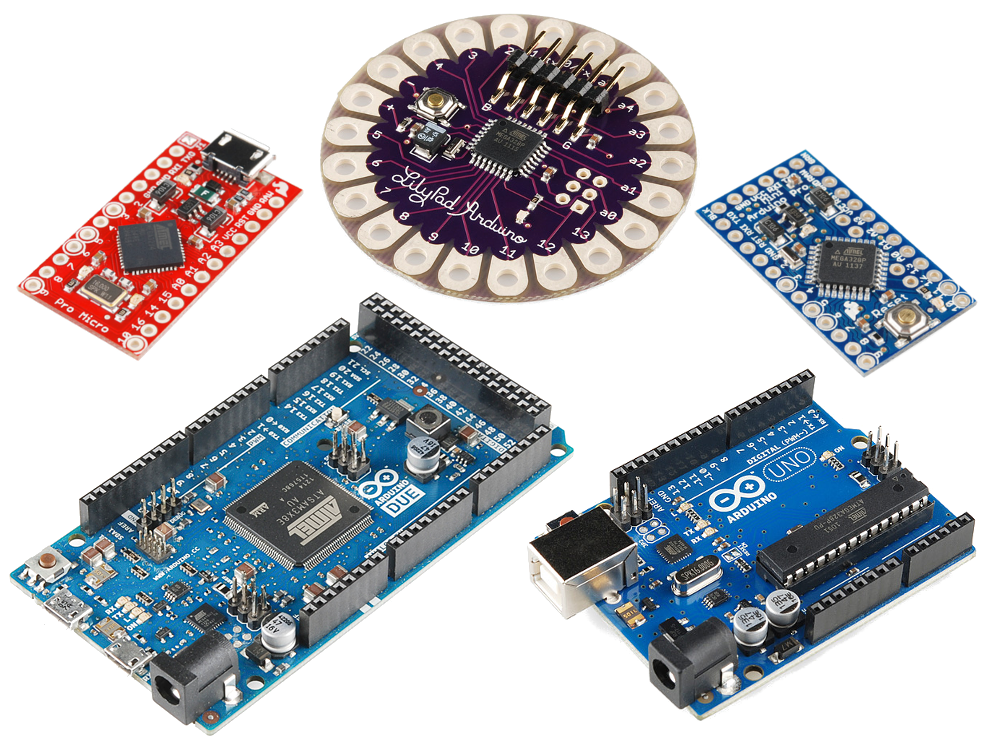
\includegraphics[height=100px]{arduinos}
\caption{ Modelos de Arduino \label{fig.arduinos} }
\end{minipage}
\begin{minipage}{0.50\textwidth}
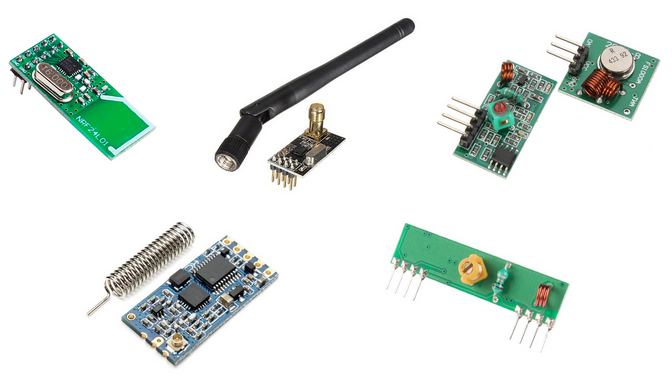
\includegraphics[height=100px]{rfs}
\caption{ Módulos RF \label{fig.rfs} }
\end{minipage}
\end{figure}

Os microcontroladores de placas compatíveis com a plataforma Arduino são os
mais populares e disponíveis no mercado brasileiro.
%
A Figura~\ref{fig.arduinos} indica alguns modelos que podem ser avaliados para
adoção no projeto (item 1).
%
Como exemplo, o modelo \emph{Pro Mini 3.3V} tem tamanho reduzido, baixo consumo
de energia e custa em torno de R\$15,00.

O levantamento, avaliação e montagem dos módulos de rádio é a etapa mais
sensível no projeto da plataforma de hardware (item 2).
%
A Figura~\ref{fig.rfs} ilustra a diversidade de módulos RF disponíveis, alguns
com custo inferior a R\$10,00.
%
Idealmente, cada um dos módulos considerados deve ser acoplável e facilmente
intercambiável na nossa plataforma, dado que temos como objetivo a
flexibilidade para experimentação e pesquisa em IoT.
%
Cada módulo poderá ser avaliado e desenvolvido em separado.
Para isso, iremos propor a exploração desses módulos em projetos da disciplina
de Software Embarcado em nosso programa de pós graduação.

%O levantamento dos microcontroladores e módulos de RF, a avaliação das
%propriedades de interesse e a prototipagem de um hardware flexível aos diversos
%módulos devem ser tema de uma dissertação de Mestrado.

A plataforma também deve permitir o acoplamento de sensores e outros
periféricos (item 3).
%
Além disso, deve oferecer mecanismos para desligá-los por software de modo a
economizar energia.
%
Esses mecanismos podem usar diretamente os pinos do microcontrolador (para
sensores mais simples) ou transistores que funcionarão como chaves eletrônicas.
%
Esse estudo pode ser realizado em separado da avaliação dos módulos de rádio
(item 2).

\begin{figure}
\begin{minipage}{0.50\textwidth}
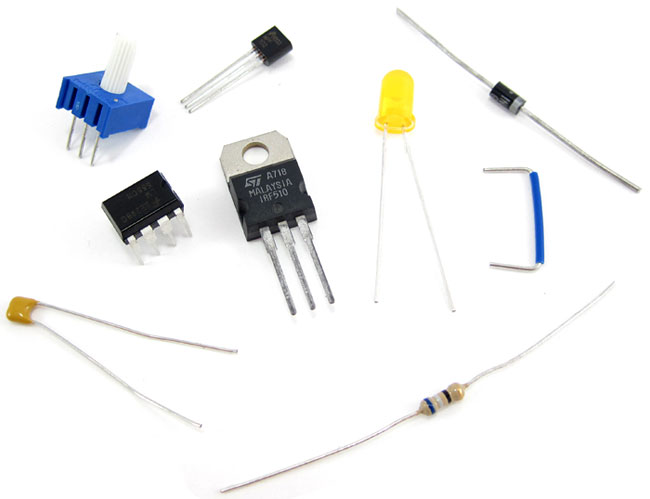
\includegraphics[height=100px]{through-hole}
\end{minipage}
\begin{minipage}{0.50\textwidth}
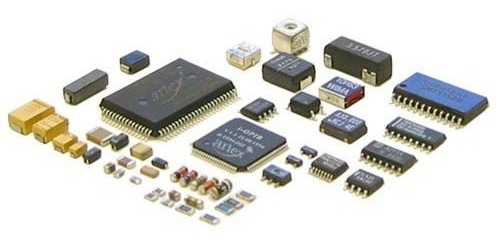
\includegraphics[height=100px]{smd}
\end{minipage}
\caption{ Componentes \emph{Through-Hole} (esquerda) e \emph{Surface-Mount} (direita).
    \label{fig.mount}
}
\end{figure}

Os componentes eletrônicos devem possuir pinos para montagem
\emph{through-hole}, como ilustrado na Figura~\ref{fig.mount}, que é a técnica
mais flexível e adequada para protótipos considerando o contexto de pesquisa.
%
Esses componentes também são mais disponíveis no mercado para compras em
pequenas quantidades.
%
Ao fim do projeto, desejamos obter um protótipo de tamanho similar aos da
Figura~\ref{fig.protos}.

\begin{figure}
\begin{minipage}{0.50\textwidth}
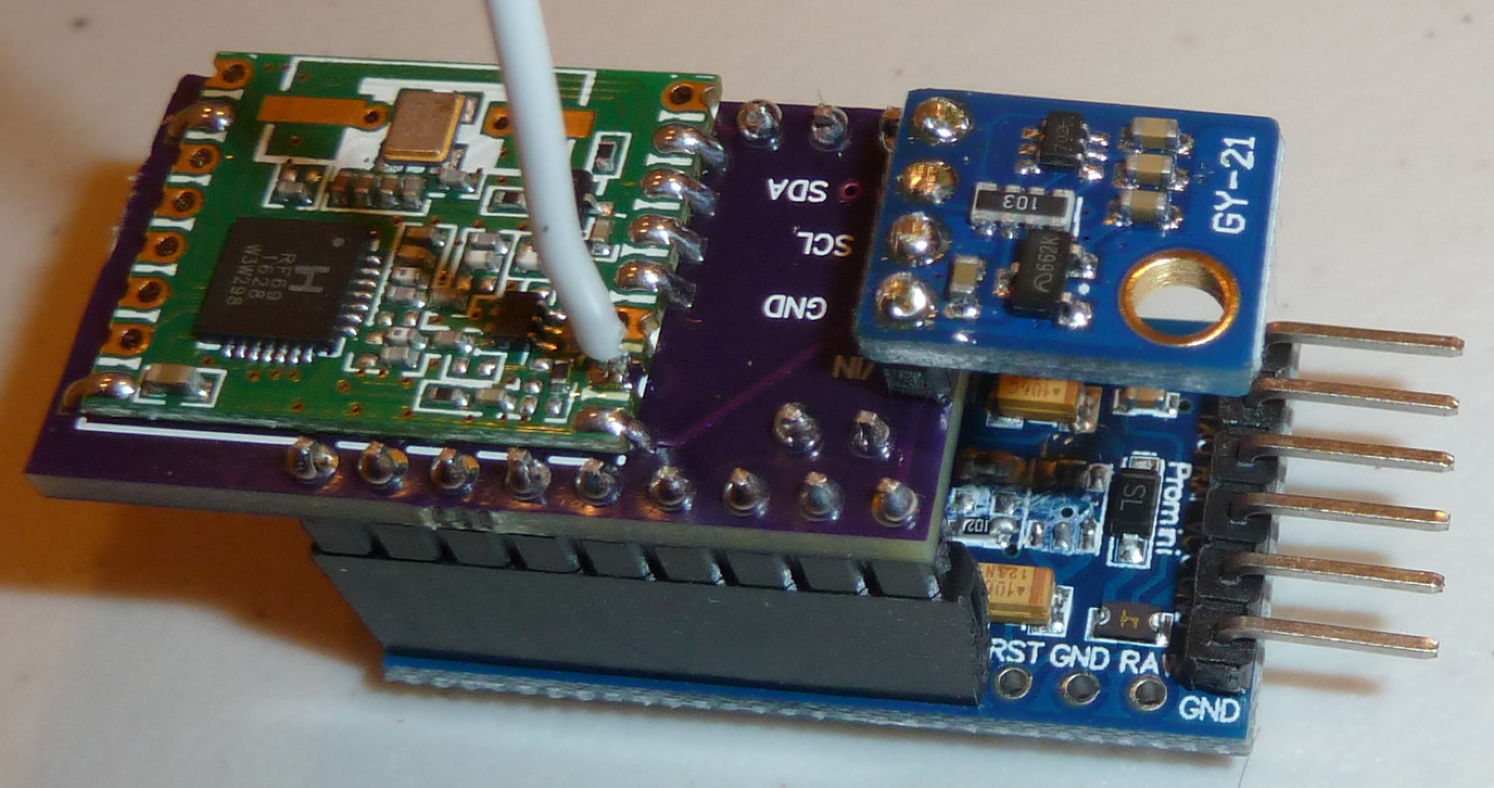
\includegraphics[height=75px]{proto-01}
\end{minipage}
\begin{minipage}{0.50\textwidth}
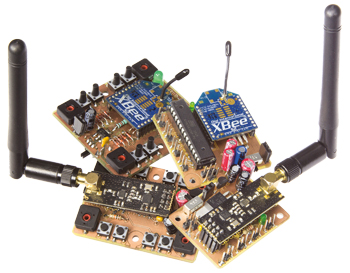
\includegraphics[height=150px]{proto-03}
\end{minipage}
\caption{ Protótipos de dispositivos IoT. \label{fig.protos} }
\end{figure}

É importante destacar que o desenvolvimento do hardware não depende da frente
de pesquisa de software em \CEU, e tampouco depende do desenvolvimento de
softwares complexos (mesmo que em outras linguagens).
Como iremos utilizar hardware de commodity, já existe oferta suficiente de
bibliotecas de software e aplicações open-source para testes.
%
Apenas para a avaliação de consumo de energia que as duas frentes deverão ser
necessariamente integradas.

%%%%%%%%%%%%%%%%%%%%%%%%%%%%%%%%%%%%%%%%%%%%%%%%%%%%%%%%%%%%%%%%%%%%%%%%%%%%%%%
% g) Etapas de execução do projeto com respectivo cronograma de atividades;
%%%%%%%%%%%%%%%%%%%%%%%%%%%%%%%%%%%%%%%%%%%%%%%%%%%%%%%%%%%%%%%%%%%%%%%%%%%%%%%

\section{ Cronograma de Atividades }

O projeto deve se estender por 2 anos (8 trimestres) conforme retratado na
Figura~\ref{fig.crono}.
%
O projeto é dividido em 5 fases:
%
\begin{description}
\item[Fase 0:]
Essa fase compreende o trabalho de infra-estrutura da linguagem \CEU.
Inclui atividades no início do projeto relativas ao suporte recente de
interrupções e gerenciamento de energia a serem finalizados.
Também inclui atividades eventuais de manutenção da linguagem durante todo o
projeto.
%
\item[Fase I:]
Essa fase compreende o levantamento de módulos de RF a serem considerados e
que em seguida farão parte de plataforma de hardware.
O primeiro protótipo de hardware já deve acomodar os diferentes módulos de RF
para testes de campo.
Por fim, faremos uma avaliação quantitativa dos módulos considerando diversas
propriedades, tais como alcance, velocidade e consumo de energia em modo ativo
(i.e., sem modo de espera).
Essa avaliação usará \emph{microbenchmarks} para as diversas propriedades e não
depende da linguagem \CEU pois usará bibliotecas já disponíveis em C.
%
\item[Fase II:]
Essa fase inclui o desenvolvimento em \CEU de drivers para os rádios e
aplicações completas de IoT, que devem ser eficientes em termos de consumo de
energia no modo de espera.
Faremos uma avaliação quantitativa do uso de recursos computacionais para as
aplicações desenvolvidas.
Esperamos obter economias de energia significativas pelo gerenciamento de
energia automático de \CEU.
%
\item[Fase III:]
Essa fase complementa as Fases I e II com outros sensores, periféricos,
mecanismos de economia de energia e também ajustes e acabamentos do protótipo.
Ao fim do projeto, esperamos ter uma solução completa de IoT de hardware e
software para um artigo de maior impacto.
%
\item[Fase IV:]
Essa fase é independente das demais e deve se estender por todo o período do
projeto.
O objetivo é avaliar qualitativamente a usabilidade de \CEU com alunos de
graduação.
Ela também vai servir para atrair novos alunos para a área de sistemas
embarcados e IoT, construir uma comunidade em torno de \CEU, e avaliar o nosso
protótipo de hardware em momentos tardios do projeto.
\end{description}

\begin{comment}
%\item[Fase 0:]
This phase constitutes the infra-structure work in the language Céu.
It includes activities in the beginning of the project related to the new
support for interrupts and energy management yet to be finalized.
It also includes bookkeeping activities in the language throughout the whole
project.

%\item[Fase I:]
This phase constitutes the study of RF modules to be considered for the
hardware platform.
The first hardware prototype should already accommodate the different RF
modules for tests.
Finally, we will make a quantitative evaluation of the modules considering
several properties, such as range, speed, and energy consumption in active mode
(i.e., without standby).
This evaluation will use microbenchmarks for the several properties and does
not depend on the language Céu because it will use existing libraries in C.

% \item[Fase II:]
This phase includes the development in Céu of the radio drivers and complete
IoT applications, which should be energy efficient in standby mode.
We will make a quantitative evaluation of the computational resources for the
applications.
We expect to obtain significant economy due to the automatic energy management
of Céu.

%\item[Fase III:]
This phase complements the previous two phases with other sensors, peripherals,
energy-efficiency mechanisms, and also adjusts in the prototype.
At the end of the project, we expect to have a complete hardware and software
IoT solution for a paper of higher impact.

%\item[Fase IV:]
This phase is independent from the others and should extend through the whole
project.
The goal is to evaluate qualitatively the usability of Céu with undergraduate
students.
It will also serve to attract new students for the area of embedded systems and
IoT, to build a community around Céu, and to evaluate our hardware prototype
later in the project.
\end{comment}

\begin{figure}[t]
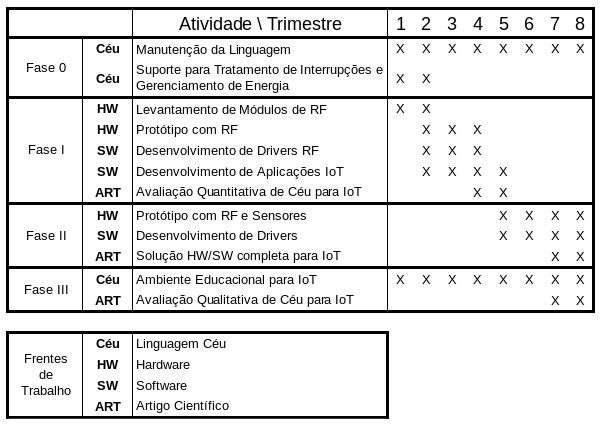
\includegraphics[width=\textwidth]{crono}
\caption{ Cronograma de Atividades \label{fig.crono} }
\end{figure}

%%%%%%%%%%%%%%%%%%%%%%%%%%%%%%%%%%%%%%%%%%%%%%%%%%%%%%%%%%%%%%%%%%%%%%%%%%%%%%%
% h) Produtos esperados como resultado da execução do projeto, com previsão de cronograma de entregas anuais;
%%%%%%%%%%%%%%%%%%%%%%%%%%%%%%%%%%%%%%%%%%%%%%%%%%%%%%%%%%%%%%%%%%%%%%%%%%%%%%%

\section{ Resultados Esperados }

Ao fim de cada semestre, esperamos obter os seguintes resultados:

\begin{itemize}
\item Primeiro Semestre:
    \begin{enumerate}
    \item Uma versão de \CEU com suporte a tratamento de interrupções e
          gerenciamento de energia automático.
    \item Uma disciplina opcional de IoT preparada para alunos no início
          da graduação usando o ambiente de programação de \CEU.
    \end{enumerate}
\item Segundo Semestre:
    \begin{enumerate}
    \item Um protótipo de hardware com suporte a diversos módulos de RF.
    \item Um artigo com o levantamento e avaliação de módulos de RF com foco em
          \emph{microbenchmarks} para consumo de energia.
    \item Um conjunto de drivers em \CEU para módulos de RF cientes de energia.
    \end{enumerate}
\item Terceiro Semestre:
    \begin{enumerate}
    \item Um artigo com a avaliação quantitativa de \CEU considerando
          aplicações completas e representativas de IoT.
    \item Um protótipo de hardware completo com módulos de RF, sensores, etc.
    \end{enumerate}
\item Quarto Semestre:
    \begin{enumerate}
    \item Um conjunto de drivers em \CEU para sensores e outros periféricos.
    \item Um artigo com a solução HW/SW completa da nossa plataforma de IoT.
    \item Um artigo com a avaliação qualitativa de usabilidade de \CEU
          considerando todo o software desenvolvido durante o projeto e também
          a nossa experiência com alunos de graduação.
    \end{enumerate}
\end{itemize}

%%%%%%%%%%%%%%%%%%%%%%%%%%%%%%%%%%%%%%%%%%%%%%%%%%%%%%%%%%%%%%%%%%%%%%%%%%%%%%%
% i) Potencial de impacto dos resultados do ponto de vista técnico-científico, de inovação, difusão, sócio-econômico e ambiental;
%%%%%%%%%%%%%%%%%%%%%%%%%%%%%%%%%%%%%%%%%%%%%%%%%%%%%%%%%%%%%%%%%%%%%%%%%%%%%%%

\section{ Potencial de Impacto }

Como destacado no resumo do projeto, o consumo de energia estimado com o
crescimento da IoT terá consequências significativas para o meio ambiente.
A nossa proposta para tratamento automático do modo de espera no nível da
linguagem de programação pode ser solução uma escalável para esse problema.
Potencialmente, todas as aplicações escritas em \CEU se beneficiariam desse
mecanismo automático, sem esforços extras de programação.

\CEU é uma linguagem que vem sendo desenvolvida pelos últimos 8 anos, desde o
início do doutorado do pesquisador proponente.
Além das nossas próprias contribuições científicas, \CEU já foi utilizada como
base para a pesquisa de terceiros~\cite{ceu.terber} e também para o
desenvolvimento de produtos na indústria de sistemas embarcados.
\CEU oferece um modelo de concorrência antagônico ao de linguagens mais
tradicionais (incluindo linguagens acadêmicas).
Isso concede a ela algumas frentes de inovação, como por exemplo o
gerenciamento automático de energia.

A nossa proposta é uma plataforma aberta tanto de software como de hardware que
pode ser reusada por outros grupos de pesquisa.
Propomos uma solução flexível para atender cenários diversos e também de baixo
custo para estimular uma maior adoção.

Um objetivo secundário do nosso trabalho é criar um ambiente de programação
para educação em IoT.
Esse ambiente será usado em um curso introdutório de IoT para alunos no início
da graduação.
Consideramos importante fomentar o interesse de alunos nesse tema o mais cedo
possível.

%%%%%%%%%%%%%%%%%%%%%%%%%%%%%%%%%%%%%%%%%%%%%%%%%%%%%%%%%%%%%%%%%%%%%%%%%%%%%%%
% n) Orçamento detalhado.
%%%%%%%%%%%%%%%%%%%%%%%%%%%%%%%%%%%%%%%%%%%%%%%%%%%%%%%%%%%%%%%%%%%%%%%%%%%%%%%

\section{ Orçamento Detalhado }

A Figura~\ref{fig.orcamento} detalha o orçamento por semestre para o período
total de 2 anos do projeto.
O orçamento total é de R\$27.420,00 divididos em recursos de capital
(R\$11.500,00) e custeio (R\$15.920,00).

Os recursos de capital se concentram no primeiro semestre, com a compra de um
notebook, monitor e osciloscópio.
Além disso, adquiriremos os componentes para o desenvolvimento da plataforma de
hardware aos poucos, ao longo dos 4 semestres.

Os recursos de custeio se concentram em viagens para eventos e congressos de
IoT e sistemas embarcados.
Esperamos ter material para até 4 artigos científicos e desejamos publicar
alguns deles em conferências para maior divulgação.
Dentre as possíveis conferências, podemos destacar o \emph{Simpósio Brasileiro
de Redes de Computadores (SBRC)}, \emph{Brazilian Symposium on Computing
Systems Engineering (SBESC)} e o \emph{ACM Conference on Embedded Networked
Sensor Systems}.
Também reservamos recursos ao longo dos 4 semestres para a confecção de placas
de circuito impresso para a plataforma de hardware.

\begin{figure}[t]
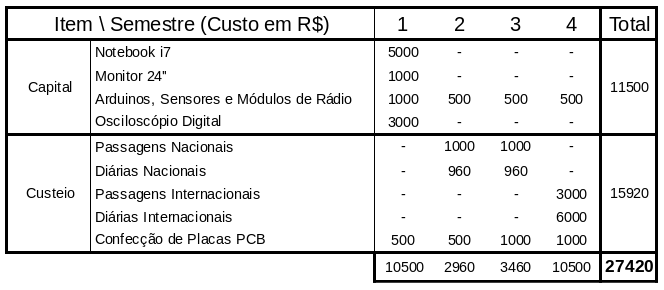
\includegraphics[width=\textwidth]{orcamento}
\caption{ Orçamento Detalhado \label{fig.orcamento} }
\end{figure}

%%%%%%%%%%%%%%%%%%%%%%%%%%%%%%%%%%%%%%%%%%%%%%%%%%%%%%%%%%%%%%%%%%%%%%%%%%%%%%%
% l) Recursos financeiros de outras fontes aprovados para aplicação no projeto;
%%%%%%%%%%%%%%%%%%%%%%%%%%%%%%%%%%%%%%%%%%%%%%%%%%%%%%%%%%%%%%%%%%%%%%%%%%%%%%%

\section{ Recursos de Outras Fontes }

O pesquisador proponente é atualmente coordenador do projeto intitulado
\emph{Energy Efficiency for IoT Software in the Large} financiado pelo
Instituto Serrapilheira em sua 1a chamada pública%
\footnote{\url{https://serrapilheira.org/chamada-publica-no1/}}.
%
O projeto conta com financiamento de R\$70.000 e tem previsão de término para
fevereiro de 2019.
%
O escopo do projeto se concentra em desenvolver novos mecanismos de eficiência
energética no nível de linguagem de programação.
%
Os recursos financeiros estão sendo usados principalmente para pagamento de
bolsas e viagens.

O novo projeto proposto neste documento é uma plataforma completa de hardware e
software que já considera os resultados obtidos no projeto em andamento,
conforme descrito no início da Seção~\ref{sec.metodologia.software}.

%%%%%%%%%%%%%%%%%%%%%%%%%%%%%%%%%%%%%%%%%%%%%%%%%%%%%%%%%%%%%%%%%%%%%%%%%%%%%%%

\begin{comment}
- Falar mais sobre ferramenta da Anny, GSoC

j) Colaborações ou parcerias já estabelecidas para a execução do projeto;
k) Perspectivas de colaborações interinstitucionais para a execução do projeto;
m) Disponibilidade efetiva de infraestrutura e de apoio técnico para o desenvolvimento do
projeto;
\end{comment}

\bibliographystyle{plain}
\bibliography{my,other,serra} 

\end{document}
